\documentclass[12pt]{article}

%==============================================
% Begin packages
%==============================================

%1:45 -- 2:35		50
%3:50 -- 3:52		52
%3:55 -- 5:55		172
%6:10 -- 6:28		190
%7:07 -- 7:19		202
%7:43 -- 7:59		218
%8:10 -- 8:34		242
%9:05 -- 9:21		258
%10:21 -- 12:50
\usepackage[margin=2cm]{geometry}
\usepackage{amsthm}
\usepackage{amsmath}
\usepackage{amssymb}
%\usepackage[charter]{mathdesign}
\usepackage[super]{nth}
\usepackage{mleftright}
\usepackage[per-mode=fraction]{siunitx}
\usepackage[shortlabels]{enumitem}
\usepackage{booktabs}
\usepackage{caption}
\usepackage{pgfplots}
\usepackage{answers}
\usepackage{hyperref}

\usepackage{cleveref} % Load last!

%==============================================
%General format settings
%==============================================

\setlength{\parindent}{0pc}
\setlength{\parskip}{1pc}

%==============================================
%Tikz settings
%==============================================

\pgfplotsset{
	compat=1.9,
    	axis x line=middle,
    	axis y line=middle,
    	xlabel=$x$,
    	ylabel=$y$,
    	xmin=-7, xmax=7,
    	ymin=-7, ymax=7,
    	xtick={},
    	ytick={},
    	minor xtick={-6,-5,...,6},
    	minor ytick={-6,-5,...,6},
    	width=0.5\linewidth,
    	height=0.5\linewidth,
    	grid=minor,
	cell picture = false,
}

%==============================================
%Exercises and solutions
%==============================================

\Newassociation{question}{Question}{questions}
\Newassociation{answer}{Answer}{answers}

%==============================================
%New environments
%==============================================

%Each lab is a section*

\newtheoremstyle{activity}% name of the style to be used
  {3pt}% measure of space to leave above the theorem. E.g.: 3pt
  {3pt}% measure of space to leave below the theorem. E.g.: 3pt
  {\mdseries}% name of font to use in the body of the theorem
  {}% measure of space to indent
  {\bfseries}% name of head font
  {{}}% punctuation between head and body
  {1pc}% space after theorem head; " " = normal interword space
  {\thmname{#1}\thmnumber{ #2}\\[0.5pc] 
     \setcounter{equation}{0} 
     \setcounter{example}{0} 
     \setcounter{definition}{0} 
     \setcounter{problem}{0}
     \setcounter{table}{0}
     \setcounter{figure}{0}}% Manually specify head
\theoremstyle{activity}
\newtheorem{activity}{Activity}

\newenvironment{intro}{}{}

\newtheoremstyle{problem}% name of the style to be used
  {3pt}% measure of space to leave above the theorem. E.g.: 3pt
  {3pt}% measure of space to leave below the theorem. E.g.: 3pt
  {\mdseries}% name of font to use in the body of the theorem
  {}% measure of space to indent
  {\bfseries}% name of head font
  {{}}% punctuation between head and body
  {1pc}% space after theorem head; " " = normal interword space
  {\thmname{#1}\thmnumber{ \theactivity.#2}}% Manually specify head
\theoremstyle{problem}
\newtheorem{problem}{Problem}


\newlist{parts}{enumerate}{4}
\setlist[parts,1,2]{label=\theactivity.\theproblem.\arabic*,%
  }

\newenvironment{hint}{{\bfseries Hint:}}{}

\newtheoremstyle{example}% name of the style to be used
  {1pc}% measure of space to leave above the theorem. E.g.: 3pt
  {3pt}% measure of space to leave below the theorem. E.g.: 3pt
  {\mdseries}% name of font to use in the body of the theorem
  {}% measure of space to indent
  {\bfseries}% name of head font
  {{}}% punctuation between head and body
  {1pc}% space after theorem head; " " = normal interword space
  {\thmname{#1}\thmnumber{ #2}}% Manually specify head
\theoremstyle{example}
\newtheorem{example}{Example}

\newtheoremstyle{definition}% name of the style to be used
  {1pc}% measure of space to leave above the theorem. E.g.: 3pt
  {3pt}% measure of space to leave below the theorem. E.g.: 3pt
  {\mdseries}% name of font to use in the body of the theorem
  {}% measure of space to indent
  {\bfseries}% name of head font
  {{}}% punctuation between head and body
  {1pc}% space after theorem head; " " = normal interword space
  {\thmname{#1}\thmnumber{ #2} \\[1pc]}% Manually specify head
\theoremstyle{definition}
\newtheorem{definition}{Definition}

\newtheoremstyle{exercises}% name of the style to be used
  {1pc}% measure of space to leave above the theorem. E.g.: 3pt
  {0pt}% measure of space to leave below the theorem. E.g.: 3pt
  {\mdseries}% name of font to use in the body of the theorem
  {}% measure of space to indent
  {\bfseries}% name of head font
  {{}}% punctuation between head and body
  {1pc}% space after theorem head; " " = normal interword space
  {\thmname{#1}\thmnumber{ #2} \\[1pc]}% Manually specify head
\theoremstyle{exercises}
\newtheorem{exercises}{Exercises}

\newtheoremstyle{exercise}% name of the style to be used
  {0pc}% measure of space to leave above the theorem. E.g.: 3pt
  {-2\parskip}% measure of space to leave below the theorem. E.g.: 3pt
  {}% name of font to use in the body of the theorem
  {}% measure of space to indent
  {}% name of head font
  {{}}% punctuation between head and body
  {0pc}% space after theorem head; " " = normal interword space
  {{}}% Manually specify head
\theoremstyle{exercise}
\newtheorem{exercise}{}




  
%==============================================
%Enumeration settings
%==============================================

\renewcommand{\thesection}{\Alph{section}}
\renewcommand{\thetable}{\theactivity.\arabic{table}}
\renewcommand{\thefigure}{\theactivity.\arabic{figure}}
\renewcommand{\theequation}{\theactivity.\arabic{equation}}
\renewcommand{\theexample}{\theactivity.\arabic{example}}
\renewcommand{\thedefinition}{\theactivity.\arabic{definition}}
\renewcommand{\theexercises}{\thesection.\arabic{exercises}}
\renewcommand{\theexercise}{\theexercises.\arabic{exercise}}
\renewcommand{\theQuestion}{\theexercises.\arabic{Question}}

%==============================================
%Cleveref
%==============================================

\crefname{equation}{Equation}{Equations} 
\Crefname{equation}{Equation}{Equations} 

\crefname{table}{Table}{Tables} 

\crefname{figure}{Figure}{Figures} 
\Crefname{figure}{Figure}{Figures} 

\crefname{parts}{Problem}{Problems} 
\Crefname{parts}{Problem}{Problems} 
\crefalias{partsi}{parts}
\crefalias{partsii}{parts}
\crefalias{partsiii}{parts}

\crefname{example}{Example}{Examples} 
\Crefname{example}{Example}{Examples} 

\crefname{definition}{Definition}{Definitions} 
\Crefname{definition}{Definition}{Definitions} 

\crefname{exercise}{Exercise}{Exercises} 
\Crefname{exercise}{Exercise}{Exercises} 

\crefname{Question}{Exercise}{Exercises} 
\Crefname{Question}{Exercise}{Exercises} 


%==============================================
%siunitx
%==============================================

\DeclareSIUnit\foot{ft}
\DeclareSIUnit\gallon{gal}

%==============================================
%Begin document
%==============================================


\begin{document}

\section{Rates of Change}
\begin{activity}{}

\begin{intro}
Motion is frequently modeled using calculus. A building block for this application is the concept of \emph{average velocity}. Average velocity is defined to be net displacement divided by elapsed time. More precisely, if $p$ is a position function for something moving along a numbered line, then we define the average velocity over the time interval $\left[t_0,t_1\right]$ to be: 
\begin{align}\label{ratesofchange:eq:avgvel}
\text{average velocity}
&=\frac{p\mleft(t_1\mright)-p\mleft(t_0\mright)}{t_1-t_0}
\end{align}
\end{intro}
%
\begin{problem}{}
According to simplified Newtonian physics, if an object is dropped from a height of \SI{200}{\meter} and allowed to free fall to the ground, then the height of the object (measure in \si{\meter}) is given by the position function $p$ where $p(t)=200-4.9t^2$ where $t$ is the amount of time that has passed since the object was dropped (measured in \si{\second}).

\begin{parts}
\item What, \emph{including units}, are the values of $p(t)$ three seconds and five seconds into the object's fall? Use these values when working \cref{ratesofchange:prob:calculate}.
\item \label{ratesofchange:prob:calculate} Calculate $\frac{p(\SI{5}{\second})-p(\SI{3}{\second})}{\SI{5}{\second}-\SI{3}{\second}}$; \emph{include units while making the calculation}. What does the result tell you in the context of this problem? 
\item  \label{ratesofchange:prob:general}Use \cref{ratesofchange:eq:avgvel} to find a formula for the average velocity of this object over the general time interval $\left[t_0,t_1\right]$. The first couple of lines of this process are shown below. Copy these lines onto your paper and continue the simplification process. 
\begin{align*}
\frac{p\mleft(t_1\mright)-p\mleft(t_0\mright)}{t_1-t_0}
&=\frac{\left[200-4.9t_1^2\right]-\left[200-4.9t_0^2\right]}{t_1-t_0}\\
&=\frac{200-4.9t_1^2-200+4.9t_0^2}{t_1-t_0}\\
&=\frac{-4.9t_1^2+4.9t_0^2}{t_1-t_0}
\end{align*}
%
\begin{hint}
In the next step you should factor $-4.9$ from the numerator; the remaining factor will factor further.
\end{hint}
\item  Check the formula you derived in \cref{ratesofchange:prob:general} using $t_0=3$ and $t_1=5$; that is, compare the value
generated by the formula to that you found in \cref{ratesofchange:prob:calculate}. 
\item Using the formula found in \cref{ratesofchange:prob:general}, replace $t_0$ with $3$ but leave $t_1$ as a variable; simplify the result. Then copy \cref{ratesofchange:tab:calculate} onto your paper and fill in the missing entries. 
\begin{table}[!ht]
\centering
\caption{$y=\frac{p_1(t)-p_1(3)}{t-3}$}\label{ratesofchange:tab:calculate}
\begin{tabular}{SS}
\toprule
{$t_1$ (\si{\second})} & {$y$ (\si{\meter\per\second})}\\
\midrule
2.9&\\
\midrule
2.99&\\
\midrule
2.999&\\
\midrule
3.001&\\
\midrule
3.01&\\
\midrule
3.1&\\
\bottomrule
\end{tabular}
\end{table}

\item As the value of $t_1$ gets closer to $3$, the values in the $y$ column of \cref{ratesofchange:tab:calculate} appear to be
converging on a single number; what is this number and what do you think it tells you in the context of this problem? 

\end{parts}

\end{problem}

\end{activity}


\begin{activity}{}
One of the building blocks in differential calculus is \emph{the secant line to a curve}. It is very easy for a line to be considered a secant line to a curve; the only requirement that must be fulfilled is that the line intersects the curve in at least two points. 

In \cref{ratesofchange:fig:secant}, a secant line to the curve $y=f(x)$ has been drawn through the points $(0,3)$ and $(4,-5)$. You should verify that the slope of this line is $-2$.

\begin{figure}[!ht]
\centering
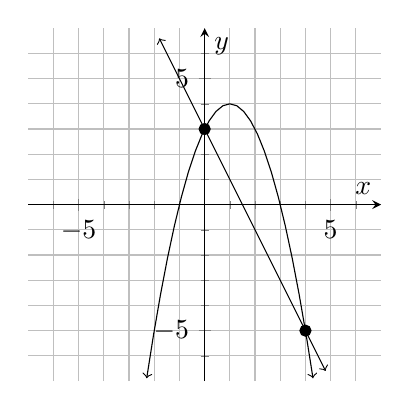
\begin{tikzpicture}
	\begin{axis}[		]
		\addplot[domain=-2.3:4.3,<->]{3+2*x-x^2};
		\addplot[domain=-1.8:4.8,<->]{3-2*x};
		\addplot[only marks] coordinates{(0,3) (4,-5)};
		\end{axis}
	\end{tikzpicture}
\caption{$y=f(x)$ and a secant line}\label{ratesofchange:fig:secant}
\end{figure}

The formula for $f$ is $f(x)=3+2x-x^2$. We can use this formula to come up with a generalized formula for the slope of secant lines to this curve. Specifically, the slope of the line connecting the point $\left(x_0,f\mleft(x_0\mright)\right)$ to the point $\left(x_1,f\mleft(x_1\mright)\right)$, is derived in \cref{ratesofchange:ex:secant}. 

\begin{example}\label{ratesofchange:ex:secant}
\begin{align*}
m_{\text{sec}}
&= \frac{f\mleft(x_1\mright)-f\mleft(x_0\mright)}{x_1-x_0}\\
&= \frac{\left(3+2x_1-x_1^2\right)-\left(3+2x_0-x_0^2\right)}{x_1-x_0}\\
&= \frac{3+2x_1-x_1^2-3-2x_0+x_0^2}{x_1-x_0}\\
&= \frac{\left(2x_1-2x_0\right)-\left(x_1^2-x_0^2\right)}{x_1-x_0}\\
&= \frac{2\left(x_1-x_0\right)-\left(x_1+x_0\right)\left(x_1-x_0\right)}{x_1-x_0}&&\parbox{15em}{This factoring technique is called \emph{factoring by grouping}}\\
&= \frac{\left[2-\left(x_1+x_0\right)\right]\left(x_1-x_0\right)}{x_1-x_0}\\
&=2-x_1-x_0\text{ for }x_1\neq x_0
\end{align*}
\end{example}

We can check our formula using the line in \cref{ratesofchange:fig:secant}. If we let $x_0=0$ and $x_1=4$ then our simplified slope formula gives us: 
\begin{align*}
2-x_1-x_0
&= 2-4-0\\
&=-2\quad\checkmark
\end{align*}

\begin{problem}{}
Let $g(x)=x^2-5$.
\begin{parts}
\item  Following \cref{ratesofchange:ex:secant}, find a formula for the slope of the secant line connecting the points $\left(x_0,f\mleft(x_0\mright)\right)$ and $\left(x_1,f\mleft(x_1\mright)\right)$. Please note that factoring by grouping will not be necessary when simplifying the expression.
\item  Check your slope formula using the two points indicated in \cref{ratesofchange:fig:problem}. That is, use the graph to find the slope between the two points and then use your formula to find the slope; make sure that the two values agree!
\begin{figure}[!ht]
\centering
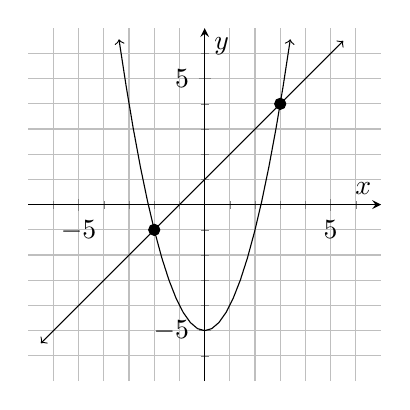
\begin{tikzpicture}
	\begin{axis}[		]
		\addplot[domain=-3.4:3.4,<->]{x^2-5};
		\addplot[domain=-6.5:5.5,<->]{1+x};
		\addplot[only marks] coordinates{(-2,-1) (3,4)};
		\end{axis}
	\end{tikzpicture}
\caption{$y=g(x)$ and a secant line}\label{ratesofchange:fig:problem}
\end{figure}

\end{parts}

\end{problem}
\end{activity}

\begin{activity}
While it's easy to see that the formula $\frac{f\mleft(x_1\mright)-f\mleft(x_0\mright)}{x_1-x_0}$ gives the slope of the line connecting two
points on the function $f$, the resultant expression can at times be awkward to work with. We actually already saw that when we had to use slight-of-hand factoring in \cref{ratesofchange:ex:secant}. 

The algebra associated with secant lines (and average velocities) can sometimes be simplified if we designate the variable $h$ to be the run between the two points (or the length of the time interval). With this designation we have $x_1-x_0=h$ which gives us $x_1=x_0+h$. Making these substitutions we get \cref{ratesofchange:eq:difquot}. The expression on the right side of \cref{ratesofchange:eq:difquot} is called \emph{the difference
quotient for $f$}.
\begin{align}\label{ratesofchange:eq:difquot}
\frac{f\mleft(x_1\mright)-f\mleft(x_0\mright)}{x_1-x_0}
&=\frac{f\mleft(x_0+h\mright)-f\mleft(x_0\mright)}{h}
\end{align} 
%
Let's revisit the function $f$ defined by $f(x)=3+2x-x^2$ from \cref{ratesofchange:ex:secant}. The difference quotient for this
function is derived in \cref{ratesofchange:ex:difquot}. 
\begin{example}\label{ratesofchange:ex:difquot}
\begin{align*}
\frac{f\mleft(x_0+h\mright)-f\mleft(x_0\mright)}{h}
&= \frac{\left[3+2\left(x_0+h\right)-\left(x_0+h\right)^2\right]-\left[3+2x_0-x_0^2\right]}{h}\\
&= \frac{3+2x_0+2h-x_0^2-2x_0h-h^2-3-2x_0+x_0^2}{h}\\
&= \frac{2h-2x_0h-h^2}{h}\\
&= \frac{h\left(2-2x_0-h\right)}{h}\\
&= 2-2x_0-h\text{ for }h\neq0
\end{align*}
\end{example}
Please notice that all of the terms without a factor of $h$ subtracted to zero. Please notice, too, that we avoided all of the tricky factoring that appeared in \cref{ratesofchange:ex:secant}! 

For simplicity's sake, we generally drop the variable subscript when applying the difference quotient. So for future reference we will define the difference quotient as follows: 

\begin{definition}{The difference quotient}
The \emph{difference quotient} for the function $f$ is the expression $\frac{f\mleft(x+h\mright)-f(x)}{h}$.
\end{definition}
\begin{problem}
Completely simplify the difference quotient for each of the following functions. Please note that the template for the difference quotient needs to be adapted to the function name and independent variable in each given equation. For example, the difference quotient for the function in \cref{ratesofchange:prob:first} is $\frac{v(t+h)-v(t)}{h}$. 
\begin{parts}
\item \label{ratesofchange:prob:first} $v(t)= 2.5t^2-7.5t$
\item $g(x)=3-7x$
\item $w(x)=\dfrac{3}{x+2}$
\end{parts}
\end{problem}

\begin{problem}
Suppose that an object is tossed into the air in such a way that the elevation of the object (measured in \si{\foot}) is given by the function
$s(t)=40+40t-16t^2$ where $t$ is the amount of time that has passed since the object was tossed (measured in \si{\second}).
\begin{parts}
\item Simplify the difference quotient for $s$.
\item \label{ratesofchange:prob:fallingdifquot} Ignoring the unit, use the difference quotient to determine the average velocity over the interval $[1.6,2.8]$. (Hint: Use $t=1.6$ and
$h=1.2$. Make sure thatyou understand why!) 
\item What, \emph{including units}, are the values of $s(1.6)$ and $s(2.8)$? Use these values when working \cref{ratesofchange:prob:fallingdifquotmore}.
\item \label{ratesofchange:prob:fallingdifquotmore} Use the expression $\frac{s(2.8)-s(1.6)}{2.8-1.6}$ to verify the value you found in \cref{ratesofchange:prob:fallingdifquot}. \emph{Include the unit while making this calculation.}
\item Ignoring the unit, use the difference quotient to determine the average velocity over the interval $[0.4,2.4]$.
\end{parts}
\end{problem}

\begin{problem}
Moose and squirrel were having casual conversation when suddenly, without any apparent provocation, Boris Badenov launched anti-moose missile in their direction. Fortunately, squirrel had ability to fly as well as great knowledge of missile technology, and he was able to disarm missile well before it hit ground. 

The elevation (\si{foot}) of the tip of the missile $t$ seconds after it was launched is given by the function $h$ defined by $h(t)=-16t^2+294.4t+15$. 
\begin{parts}
\item What, including the unit, is the value of $h(12)$ and what does the value tell you about the flight of the missile? 
\item What, including the unit, is the value of $\frac{h(\SI{12}{\second})-h(\SI{0}{\second})}{\SI{12}{\second}}$ and what does this value tell you about the flight of the missile? 
\item  The velocity (\si{\foot\per\second}) function for the missile is given by the function $v$ where $v(t)=-32t+294.4$. What, including unit, is the value of $\frac{v(\SI{10}{\second})-v(\SI{0}{\second})}{\SI{10}{\second}}$ and what does this value tell you about the flight of the missile? 
\end{parts}
\end{problem}

\begin{problem}
Timmy lived a long life in the \nth{19} century. When Timmy was seven he found a rock that weighed exactly half a stone. (Timmy lived in jolly old England, don?t you know.) That rock sat on Timmy's window sill for the next 80 years and wouldn?t you know the weight of that rock did not change even one smidge the entire time. In fact, the weight function for this rock was $w(t)=0.5$ where $w(t)$ was the weight of the rock (stones) and $t$ was the number of years that had passed since that day Timmy brought the rock home. 
\begin{parts}
\item What was the average rate of change in the weight of the rock over the 80 years it sat on Timmy's window sill? 
\item Ignoring the unit, simplify the expression $\frac{w\mleft(t_1\mright)-w\mleft(t_0\mright)}{t_1-t_0}$. Does the result make sense in
the context of this problem?
\item Showing each step in the process and ignoring the unit, simplify the difference quotient for $w$. Does the result make sense in
the context of this problem?
\end{parts}
\end{problem}

\begin{problem}
Truth be told, there was one day in 1842 when Timmy's mischievous son Nigel took that rock outside and chucked it into the air. The
velocity of the rock (\si{\foot\per\second}) was given by $v(t)=60-32t$ where $t$ was the number of seconds that had passed since Nigel chucked the rock. 
\begin{parts}
\item What, including the unit, are the values of $v(0)$, $v(1)$, and $v(2)$ and what do these values tell you in the context of this problem? Don't just write that the values tell you the velocity at certain times; explain what the velocity values tell you about the motion of the rock. 
\item Ignoring the unit, simplify the difference quotient for $v$.
\item  What is the unit for the difference quotient for $v$? What does the value of the difference quotient (including unit) tell you in
the context of this problem?  
\end{parts}
\end{problem}

\begin{problem}
Suppose that a vat was undergoing a controlled drain and that the amount of fluid left in the vat (\si{\gallon}) was given by the formula $V(t)=100-2t^{3/2}$ where $t$ is the number of minutes that had passed since the draining process began. 
\begin{parts}
\item What, including a unit, is the value of $V(4)$ and what does that value tell you in the context of this problem? 
\item Ignoring the unit, write down the formula you get for the difference quotient of $V$ when $t=4$. Copy \cref{ratesofchange:tab:vat} onto your paper and fill in the missing values. Look for a pattern in the output and write down enough digits for each entry so that the pattern is clearly illustrated; the first two entries in the output column have been given to help you understand what is meant by this direction.
\begin{table}[!ht]
\centering
\caption{$y=\frac{V(4+h)-V(4)}{h}$}\label{ratesofchange:tab:vat}
\begin{tabular}{SS}
\toprule
{$h$ (\si{\second})} & {$y$ (\si{\meter\per\second})}\\
\midrule
-0.1&-5.962\\
\midrule
-0.01&-5.9962\\
\midrule
-0.001&\\
\midrule
0.001&\\
\midrule
0.01&\\
\midrule
0.1&\\
\bottomrule
\end{tabular}
\end{table}
\item  What is the unit for the $y$-values in \cref{ratesofchange:tab:vat}? What do these values (with their unit) tell you in the context of this problem?
\item As the value of $h$ gets closer to $0$, the values in the $y$ column of \cref{ratesofchange:tab:vat} appear to be converging to a single number; what is this number and what do you think that value (with itsunit) tells you in the context of this problem? 
\end{parts}
\end{problem}
\end{activity}






\setcounter{table}{0}
\setcounter{figure}{0}
\renewcommand{\thetable}{\thesection.\arabic{table}}
\renewcommand{\thefigure}{\thesection.\arabic{figure}}

\subsection*{Supplemental Exercises}


\Opensolutionfile{questions}[questions1]
\Opensolutionfile{answers}[answers1]
\begin{exercises}
The function $z$ shown in \cref{ratesofchange:fig:z} was generated by the formula $y=2+4x-x^2$.

\begin{minipage}[t]{0.5\linewidth}
\vspace{0pt}
\centering
\captionof{table}{$y=\frac{z(4+h)-z(4)}{h}$}\label{ratesofchange:tab:z}
\begin{tabular}{SS}
\toprule
{$h$} & {$y$}\\
\midrule
-0.1&-3.9\\
\midrule
-0.01&\\
\midrule
-0.001&\\
\midrule
0.001&\\
\midrule
0.01&\\
\midrule
0.1&\\
\bottomrule
\end{tabular}
\end{minipage}
\begin{minipage}[t]{0.5\linewidth}
\vspace{0pt}
\centering
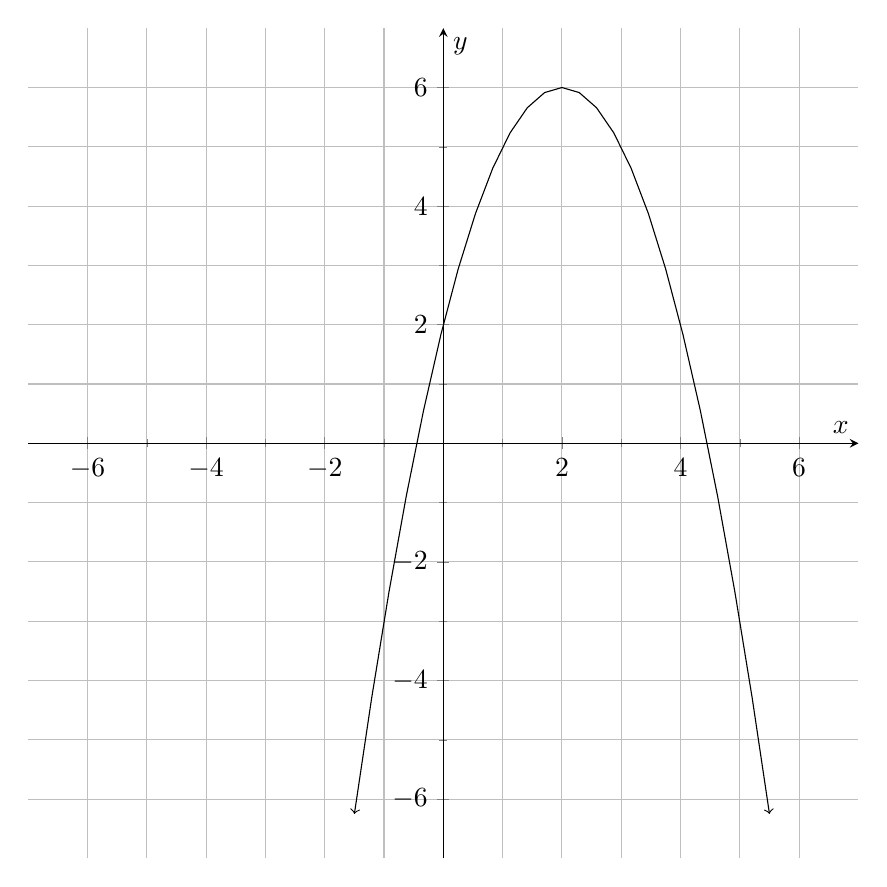
\begin{tikzpicture}
	\begin{axis}[width = \linewidth, height = \linewidth		]
		\addplot[domain=-1.5:5.5,<->]{2+4*x-x^2};
		\end{axis}
	\end{tikzpicture}
\captionof{figure}{$y=2+4x-x^2$}\label{ratesofchange:fig:z}
\end{minipage}
%
\begin{exercise} 
\begin{question}
Simplify the difference quotient for $z$.
\end{question}
\begin{answer}
The difference quotient for $z$ is:
\begin{align*}
\frac{z\mleft(x+h\mright)-z(x)}{h}
&=\frac{\left[2+4\left(x+h\right)-\left(x+h\right)^2\right]-\left[2+4x-x^2\right]}{h}\\
&=\frac{2+4x+4h-x^2-2xh-h^2-2-4x+x^2}{h}\\
&=\frac{4h-2xh-h^2}{h}\\
&=\frac{h\left(4-2x-h\right)}{h}\\
&=4-2x-h
\end{align*}
\end{answer}
\end{exercise}
%
\begin{exercise}
\begin{question}
Use the graph to find the slope of the secant line to $z$ between the points where $x=-1$ and $x=2$. Check your simplified difference quotient for $z$ by using it to find the slope of the same secant line.
\end{question}
\begin{answer}
The rise between the two points is $9$ and the run is $3$, so the slope between the two points is given by $\frac93=3$.

Using the difference quotient, if we let $x=-1$ and $h=3$ we get: 
\begin{align*}
4-2x-h
&=4-2(-1)-3\\
&=3\quad\checkmark
\end{align*}
\end{answer}
\end{exercise}
%
\begin{exercise}
\begin{question}
Replace $x$ with $4$ in your difference quotient formula and simplify the result. Then copy \cref{ratesofchange:tab:z} onto your paper and fill in the missing values. 
\end{question}
\begin{answer}
\begin{minipage}[t]{0.5\linewidth}
\vspace{0pt}
\begin{align*}
\frac{z\mleft(4+h\mright)-z(4)}{h}
&=4-2(4)-h\\
&=-4-h
\end{align*}
\end{minipage}
\begin{minipage}[t]{0.5\linewidth}
\vspace{0pt}\centering
\captionof{table}{$y=\frac{z(4+h)-z(4)}{h}$}\label{ratesofchange:tab:zsol}
\begin{tabular}{SS}
\toprule
{$h$} & {$y$}\\
\midrule
-0.1&-3.9\\
\midrule
-0.01&-3.99\\
\midrule
-0.001&-3.999\\
\midrule
0.001&-4.001\\
\midrule
0.01&-4.01\\
\midrule
0.1&-4.1\\
\bottomrule
\end{tabular}
\end{minipage}

\end{answer}
\end{exercise}
%
\begin{exercise}
\begin{question}
\label{ratesofchange:exert:hto0} As the value of $h$ gets closer to $0$, the values in the $y$ column of \cref{ratesofchange:tab:z} appear to be converging on a single number; what is this number? 
\end{question}
\begin{answer}
The values are converging on $-4$. 
\end{answer}
\end{exercise}
%
\begin{exercise}
\begin{question}
The value found in \cref{ratesofchange:exert:hto0} is called \emph{the slope of the tangent line to $z$ at $4$}. Draw onto \cref{ratesofchange:fig:z} the line that passes through the point $(4,2)$ with this slope. The line you just drew is called \emph{the tangent line to $z$ at $4$}. 
\end{question}
\begin{answer}
\begin{minipage}[t]{0.5\linewidth}
\vspace{0pt}
\centering
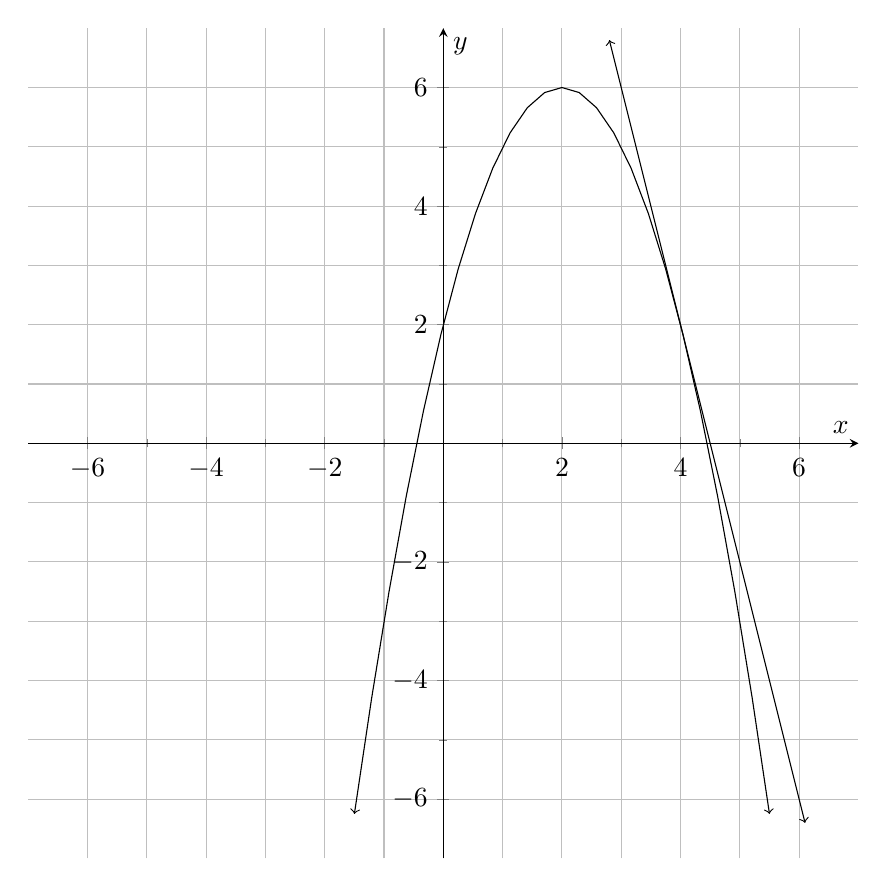
\begin{tikzpicture}
	\begin{axis}[width = \linewidth, height = \linewidth		]
		\addplot[domain=-1.5:5.5,<->]{2+4*x-x^2};
		\addplot[domain=2.8:6.1,<->]{2-4*(x-4)};
		\end{axis}
	\end{tikzpicture}
\captionof{figure}{$y=2+4x-x^2$}\label{ratesofchange:fig:z}
\end{minipage}

\end{answer}
\end{exercise}
\Closesolutionfile{questions}
\Closesolutionfile{answers}
%
\end{exercises}
\begin{Question}{A.1.1}
Simplify the difference quotient for $z$.
\end{Question}
\begin{Question}{A.1.2}
Use the graph to find the slope of the secant line to $z$ between the points where $x=-1$ and $x=2$. Check your simplified difference quotient for $z$ by using it to find the slope of the same secant line.
\end{Question}
\begin{Question}{A.1.3}
Replace $x$ with $4$ in your difference quotient formula and simplify the result. Then copy \cref{ratesofchange:tab:z} onto your paper and fill in the missing values.
\end{Question}
\begin{Question}{A.1.4}
\label{ratesofchange:exert:hto0} As the value of $h$ gets closer to $0$, the values in the $y$ column of \cref{ratesofchange:tab:z} appear to be converging on a single number; what is this number?
\end{Question}
\begin{Question}{A.1.5}
The value found in \cref{ratesofchange:exert:hto0} is called \emph{the slope of the tangent line to $z$ at $4$}. Draw onto \cref{ratesofchange:fig:z} the line that passes through the point $(4,2)$ with this slope. The line you just drew is called \emph{the tangent line to $z$ at $4$}.
\end{Question}


\setcounter{table}{0}
\setcounter{figure}{0}

\subsection*{Solutions to Supplemental Exercises}
\begin{Answer}{A.1.1}
The difference quotient for $z$ is:
\begin{align*}
\frac{z\mleft(x+h\mright)-z(x)}{h}
&=\frac{\left[2+4\left(x+h\right)-\left(x+h\right)^2\right]-\left[2+4x-x^2\right]}{h}\\
&=\frac{2+4x+4h-x^2-2xh-h^2-2-4x+x^2}{h}\\
&=\frac{4h-2xh-h^2}{h}\\
&=\frac{h\left(4-2x-h\right)}{h}\\
&=4-2x-h
\end{align*}
\end{Answer}
\begin{Answer}{A.1.2}
The rise between the two points is $9$ and the run is $3$, so the slope between the two points is given by $\frac93=3$.

Using the difference quotient, if we let $x=-1$ and $h=3$ we get:
\begin{align*}
4-2x-h
&=4-2(-1)-3\\
&=3\quad\checkmark
\end{align*}
\end{Answer}
\begin{Answer}{A.1.3}
\begin{minipage}[t]{0.5\linewidth}
\vspace{0pt}
\begin{align*}
\frac{z\mleft(4+h\mright)-z(4)}{h}
&=4-2(4)-h\\
&=-4-h
\end{align*}
\end{minipage}
\begin{minipage}[t]{0.5\linewidth}
\vspace{0pt}\centering
\captionof{table}{$y=\frac{z(4+h)-z(4)}{h}$}\label{ratesofchange:tab:zsol}
\begin{tabular}{SS}
\toprule
{$h$} & {$y$}\\
\midrule
-0.1&-3.9\\
\midrule
-0.01&-3.99\\
\midrule
-0.001&-3.999\\
\midrule
0.001&-4.001\\
\midrule
0.01&-4.01\\
\midrule
0.1&-4.1\\
\bottomrule
\end{tabular}
\end{minipage}

\end{Answer}
\begin{Answer}{A.1.4}
The values are converging on $-4$.
\end{Answer}
\begin{Answer}{A.1.5}
\begin{minipage}[t]{0.5\linewidth}
\vspace{0pt}
\centering
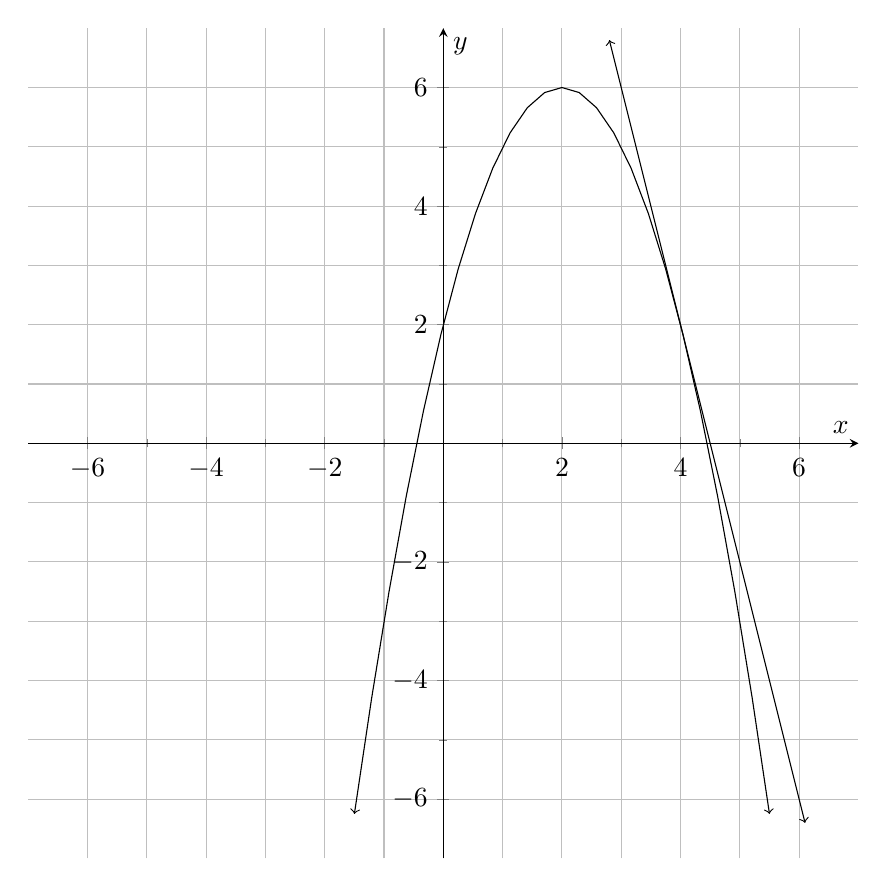
\begin{tikzpicture}
	\begin{axis}[width = \linewidth, height = \linewidth		]
		\addplot[domain=-1.5:5.5,<->]{2+4*x-x^2};
		\addplot[domain=2.8:6.1,<->]{2-4*(x-4)};
		\end{axis}
	\end{tikzpicture}
\captionof{figure}{$y=2+4x-x^2$}\label{ratesofchange:fig:z}
\end{minipage}

\end{Answer}


\end{document}